\documentclass[submission,copyright,creativecommons]{eptcs}
\providecommand{\event}{TTC 2013} 

\def\titlerunning{Petri Nets to Statecharts}
\def\authorrunning{P. {Van Gorp} and L.M. Rose}

\usepackage{url}
\usepackage{graphicx}
\usepackage{courier}
\usepackage{color}
\usepackage{listings}


\title{The Petri Nets to Statecharts Transformation Case}

\author{Pieter Van Gorp \institute{Eindhoven University of Technology, PO Box 513, 5600 MB Eindhoven, The Netherlands.} \email{p.m.e.v.gorp@tue.nl} \and Louis M. Rose \institute{Department of Computer Science, University of York, UK.} \email{louis.rose@york.ac.uk}}

\begin{document}
\maketitle

\begin{abstract}

\end{abstract}

TODO:
\begin{itemize}
  \item Abstract
  \item Add a running example to the transformation section?
  \item Evaluation criteria
  \item Break down into sub-tasks. A possible ordering:
    \subitem initialisation
    \subitem transition precedence
    \subitem OR rules
    \subitem AND rules
    \subitem Put it all together
\end{itemize}

\section{Introduction}

\section{The Transformation}
This section details the Petri net to state chart transformation algorithm, originally described by Eshuis \cite{eshuis09translating}. The transformation described below is \emph{input-destructive} (elements of the Petri net model are removed as the transformation proceeds), and uses the metamodels shown in figure~\ref{fig:mms}.

\begin{figure}[tb]
\centerline{
\begin{tabular}{c||c}
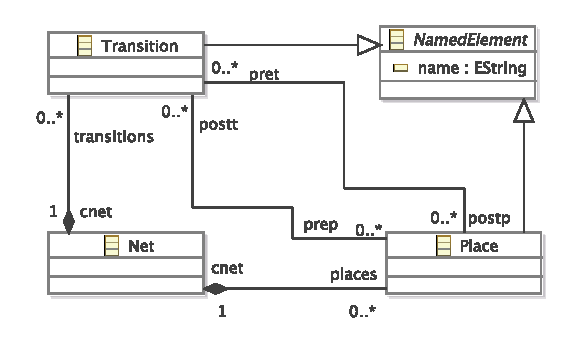
\includegraphics[width=0.45\linewidth]{images/PetriNets} & 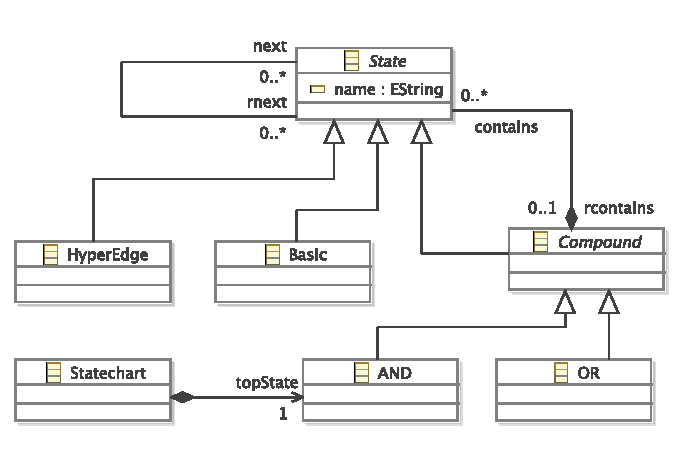
\includegraphics[width=0.5\linewidth]{images/StateCharts}\tabularnewline
(a) Petri net metamodel & (b) State chart metamodel \tabularnewline
\end{tabular}
}
\caption{\label{fig:mms}The metamodels used in the PN2SC transformation.}
\end{figure}

\subsection{Initialisation}
The first step in the PN2SC transformation involves creating an initial structure for the state chart model. In particular, the following state chart model elements are created:

\begin{itemize}
  \item For every \texttt{Place} in the Petri net:
    \subitem an instance of \texttt{Basic}, $b$
    \subitem an instance of \texttt{OR}, $o$ such that $o.contains = \{b\}$.
  \item A single instance of \texttt{Statechart}, $s$
  \item A single instance of \texttt{AND}, $a$ such that:
    \subitem $s.topstate = a$
    \subitem $\forall o: o.rcontains = a$ (i.e., every instance of \texttt{OR} is contained in $a$)
\end{itemize}

\paragraph{Equivalence.} Initialisation should also provide a mechanism for identifying the \texttt{OR} node created for a particular \texttt{Place}. The precise mechanism can vary over implementations. One approach is to use a name-based identification (i.e., assign all \texttt{Places} a uniquely identifying name and copy eaach \texttt{Place's} name to its \texttt{OR} node during initialisation.) In the remainder of this section we assume that the initialisation of the transformation will construct an injective function $equiv : Place \to OR$.

\subsection{Reduction rules}
Following initialisation, the transformation continues by applying one of two types of reduction rule: AND and OR. This section describes these two types of reduction rule, after briefly discussing the order in which the rules should be applied. 

\subsubsection{Precedence}
Correctness of the PN2SC transformation necessitates two types of precedence for the application of the AND and OR merging rules. Firstly, transitions that are more deeply nested take precedence over less nested transitions, as described below. Secondly, AND reductions always take precedence over OR reductions.

A (partial) ordering of transitions can be computed by using the ordering constraint, $\prec$, described by Eshuis \cite{eshuis09translating}. For the transitions $t_1$ and $t_2$: $t_1 \prec t_2 \Rightarrow (t_1.prep \subset t_2.postp \lor t_1.postp \subset t_2.prep)$, where $\subset$ is used to mean a strict and non-empty subset. A transition $t$ can be reduced (using the AND and OR rules described below) iff there exists no other transition $t'$ such that $t' \prec t$. Figure~\ref{fig:eol-precedence} shows an implementation of the $\prec$ in the Epsilon Object Language \cite{kolovos06eol} (a reworking and extension of OCL).

\begin{figure}
{\tiny 
\lstset{escapeinside={(*@}{@*)}}
\definecolor{gray}{rgb}{0.5,0.5,0.5}
\lstset{numbers=left,numbersep=3pt,numberstyle=\tiny,stringstyle={\color{gray}},basicstyle=\tiny,breaklines=true,emph={while,var,false,true,new,for,if,break,not,and,or,operation,Boolean,return, delete,self},emphstyle=\textbf,morecomment=[l][\color{gray}\textit]{//},morestring=[b]",showstringspaces=false,tabsize=2}
\tt
\begin{lstlisting}
operation Transition precedes?(other : Transition) : Boolean {
	if (self == other) return false;
	
	return self.prep.subset?(other.postp) or
          self.postp.subset?(other.prep));
}

operation Collection subset?(other : Collection) : Boolean {
	if (self.isEmpty()) return false;

	// (non-strict subset and not equal) => strict subset
	return other.includesAll(self) and not other.asSet().equals(self.asSet());
}
\end{lstlisting}
\rm
}{\tiny \par}

\caption{\label{fig:eol-precedence}EOL code for computing the precedence of transitions.}

\end{figure}


\begin{figure}[tb]
\centerline{
\begin{tabular}{c||c}
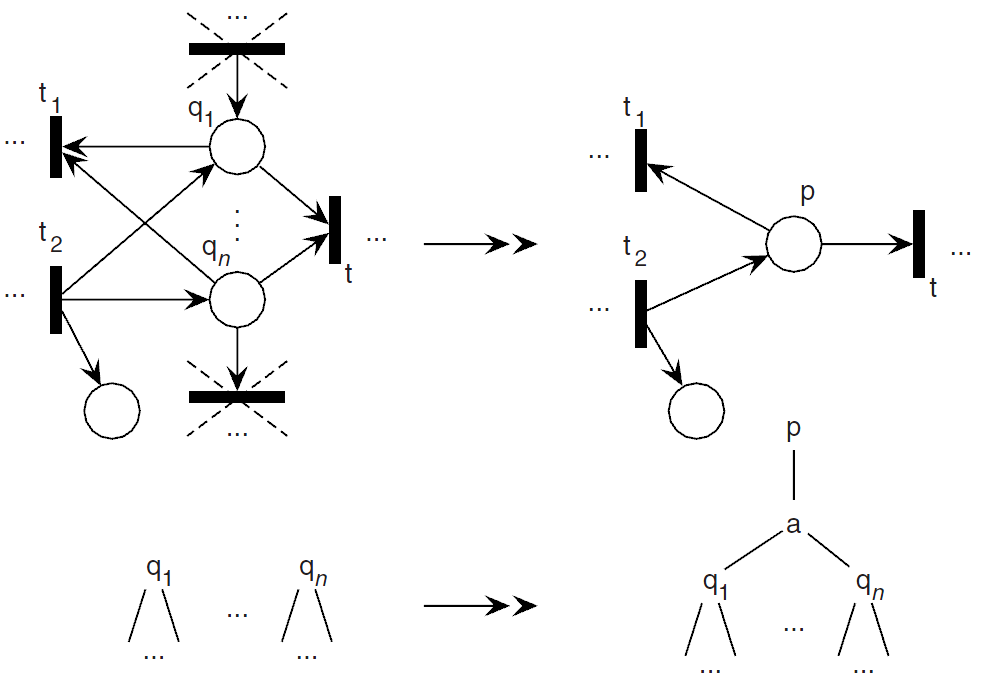
\includegraphics[width=0.45\linewidth]{images/figs-R1a} & 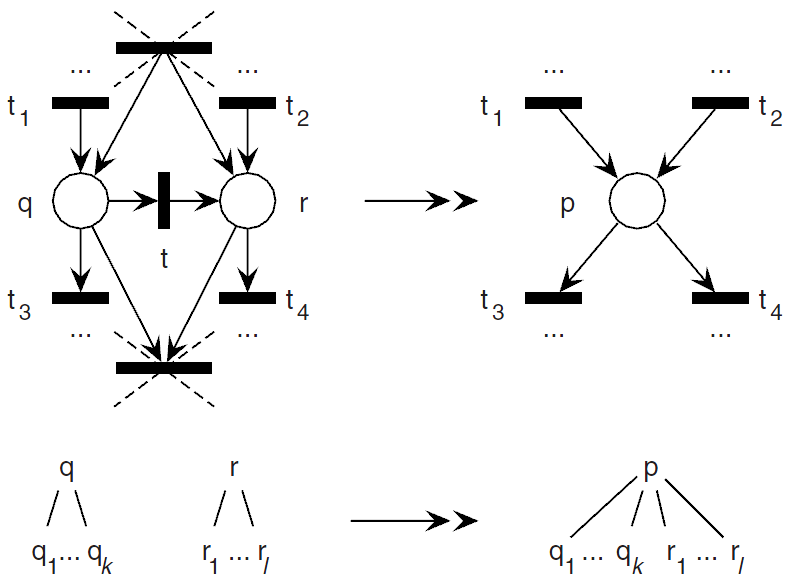
\includegraphics[width=0.5\linewidth]{images/figs-R2}\tabularnewline
(a) rule for creating \emph{AND nodes} & (b) rule for merging \emph{OR nodes}\tabularnewline
\end{tabular}
}
\caption{\label{fig:Visual-documentation-for-rules}Visual documentation for mapping rules.}
\end{figure}

\subsubsection{AND rules}
The first type of reduction rule, AND (figure~\ref{fig:Visual-documentation-for-rules}.a), constructs an \texttt{AND} state for a set of \texttt{Places} that are connected to the same incoming and outgoing \texttt{Transitions}.

\paragraph{Pre-conditions.} The AND rule can be applied to a \texttt{Transition}, $t$, iff $\left|t.prep\right| > 1$ and every \texttt{Place} in $t.prep$ is connected to the same set of outgoing transitions and the same set of incoming transitions. Alternatively, the AND rule can be applied to a \texttt{Transition}, $t$ iff
$\left|t.postp\right| > 1$ and every \texttt{Place} in $t.postp$ is connected to the same set of outgoing transitions and the same set of incoming transitions.

\paragraph{Effect on statechart.} Applying the AND rule results in the creation of a new \texttt{AND} state ($a$) and a new \texttt{OR} state ($p$) such that $p.contains = {a}$ and $a.contains$ is the set of \texttt{OR} states $\{q \in t.prep : equiv(q) \}$; or $\{q \in t.postp : equiv(q) \}$ if the rule has been applied to the transition's postset, $t.postp$.

\paragraph{Effect on Petri net.} Applying the AND rule removes from the Petri net all but one of the \texttt{Places} in the set $t.prep$ ($t.postp$).

\paragraph{EOL Implementation.} Figure~\ref{fig:eol-merge-and} shows an implementation of the AND rule in EOL. Note that the AND rule can be applied in ``both directions'' on line 2.

\begin{figure}
{\tiny \lstset{escapeinside={(*@}{@*)}}

\definecolor{gray}{rgb}{0.5,0.5,0.5}
\lstset{numbers=left,numbersep=3pt,numberstyle=\tiny,stringstyle={\color{gray}},basicstyle=\tiny,breaklines=true,emph={while,var,false,true,new,for,if,break,not,and,or,operation,Boolean,return, delete,self},emphstyle=\textbf,morecomment=[l][\color{gray}\textit]{//},morestring=[b]",showstringspaces=false,tabsize=2}
\tt
\begin{lstlisting}
operation PN!Transition apply_and_rule() : Boolean {
	return self.apply_and_rule(self.prep) or self.apply_and_rule(self.postp);
}

operation PN!Transition apply_and_rule(places : Collection(PN!Place)) : Boolean {
	var result = false;
	
	// Check pre-conditions
	if (places.size() > 1 and places.forAll(p|p.has_same_transitions_as?(places.first))) {
	  
	  // Alter statechart
		var parent = new SC!AND;
		parent.contains.addAll(places.equivalent());
		
		var root = new SC!OR;
		get_top_state().contains.add(root);		
		root.contains.add(parent);
		
		// Alter Petri net
		delete places.tail();
		
		result = true;
	}
	
	return result;
}

operation PN!Place has_same_transitions_as?(other : PN!Place) : Boolean {
	return self.pret.size() == other.pret.size() and
	       self.postt.size() == other.postt.size() and
	       self.pret.forAll(e|other.pret.includes(e)) and
	       self.postt.forAll(e|other.postt.includes(e));
}

operation Collection tail() : Collection {
	var tailed = self.clone();
	tailed.removeAt(0);
	return tailed;
}

operation PN!Place equivalent() : SC!OR {
	// This operation is implementation-specific.
	// In our solution, we use the names of Places and OR
	// nodes to implement equivalence, but other approaches
	// are equally valid and correct.
}
\end{lstlisting}
\rm
}{\tiny \par}

\caption{\label{fig:eol-merge-and}EOL code for performing AND merges (Figure~\ref{fig:Visual-documentation-for-rules}a).}

\end{figure}

\subsubsection{OR rules}
The second type of reduction rule, OR (figure~\ref{fig:Visual-documentation-for-rules}.b), constructs an \texttt{OR} state for a \texttt{Transition} that has a single preceding \texttt{Place} and single succeeding \texttt{Place}.

\paragraph{Pre-conditions.} The OR rule can be applied to a \texttt{Transition}, $t$, iff $(\left|t.prep\right| = 1) \land (\left|t.postp\right| = 1)$ and there is no transition, $t'$, such that $(q \in t'.prep) \land (r \in t'.prep)$ or $(q \in t'.postp) \land (r \in t'.postp)$ where $q$ is the single place contained in $t.prep$ and $r$ is the single place contained in $t.postp$.

\paragraph{Effect on statechart.} Applying the OR rule results in the creation of a new \texttt{OR} state ($p$) such that $p.contains$ is the set of \texttt{OR} states $equiv(q).contains \cup equiv(r).contains$.

\paragraph{Effect on Petri net.} Applying the OR rule removes from the Petri net the \texttt{Transition} $t$ and the \texttt{Places} $q$ and $r$; and adds a new \texttt{Place} $p$ such that $p.pret = (q.pret \cup r.pret)$ and $p.postt = (q.postt \cup r.postt)$.

\paragraph{EOL Implementation.} Figure~\ref{fig:eol-merge-or} shows an implementation of the OR rule in EOL. Note that this implementation re-uses $q$ to form $p$, rather than instantiate a new \texttt{Place} or \texttt{OR} state.

\begin{figure}
{\tiny \lstset{escapeinside={(*@}{@*)}}

\definecolor{gray}{rgb}{0.5,0.5,0.5}
\lstset{numbers=left,numbersep=3pt,numberstyle=\tiny,stringstyle={\color{gray}},basicstyle=\tiny,breaklines=true,emph={while,var,false,true,new,for,if,break,not,and,or,operation,Boolean,return, delete,self},emphstyle=\textbf,morecomment=[l][\color{gray}\textit]{//},morestring=[b]",showstringspaces=false,tabsize=2}
\tt
\begin{lstlisting}
operation Transition apply_or_rule() : Boolean {
	var result = false;
	
	if (self.prep.size() == 1 and self.postp.size() == 1) {
		var q = self.prep.first;
		var r = self.postp.first;
	
		if ((q == r) or not q.shares_a_transition_with?(r)) {		
			if (q <> r) {
			  var merger = q.equivalent();
  			var mergee = r.equivalent();
  			
				// Update statechart, re-using the q state as p
				merger.contains.addAll(mergee.contains);	
				delete mergee;
				
				// Update Petri net, re-using the q place as p
				q.pret.addAll(r.pret);
				q.postt.addAll(r.postt);
				delete r;
				delete self;
				
				result = true;
			}
		}
	}

	return result;
}

operation Place shares_a_transition_with?(other : Place) : Boolean {
	return self.pret.exists(e|e.postp.includes(other)) or 
	       self.postt.exists(e|e.prep.includes(other));
}

\end{lstlisting}
\rm
}{\tiny \par}

\caption{\label{fig:eol-merge-or}EOL code for performing OR merges (Figure~\ref{fig:Visual-documentation-for-rules}b).}

\end{figure}

\subsection{Termination}
The transformation proceeds by applying AND or OR rules until no \texttt{Transitions} remain in the Petri net (success) or until no further AND or OR rules can be applied (failure). The transformation might fail if the input Petri net is not well-formed.

\section{Evaluation Criteria}


\vspace{5mm}
\textbf{Acknowledgements}: The authors thank Prof. Juan de Lara for constructing the initial versions of the Petri net and state charts metamodels used in this case.

\bibliography{pn2sc}
\bibliographystyle{eptcs}

\end{document}